%!TEX root = ../../main.tex

\chapter{Kontextabgrenzung}
Die Kontextabgrenzung beschäftigt sich mit den Schnittstellen zu eCourse.
eCourse wird als \gls{Standalone}-Anwendung entwickelt. Daher entstehen keine externen Abhängigkeiten zu anderen Anwendungen und es fließen auch keine Daten zwischen eCourse und anderen Anwendungen. \\
Daher kann auf eine eingehende Betrachtung der Schnittstellen und des Datenflusses verzichtet werden. In Abbildung \ref{fib:Kontext} ist die Beziehung zwischen eCourse und anderen Anwendungen nochmals graphisch dargestellt. 
\begin{figure}[H]
\centering
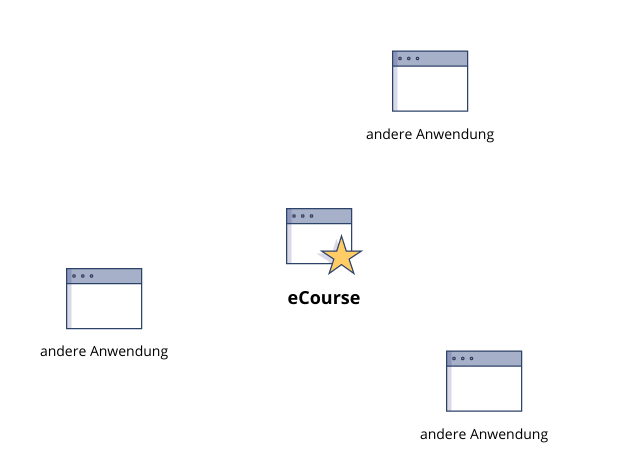
\includegraphics[height=.4\textwidth]{Kontextdiagramm.png}
\caption{Kontextdiagramm für die Anwendung eCourse}
\label{fib:Kontext}
\end{figure}